\section[连续时间中的随机过程]{连续时间中的随机过程\\Random Processes in Continuous Time}
	\subsection{连续时间中的随机过程}
	
	到目前为止,我们认为观测的顺序无关紧要,我们收集了所有的观测数据,通过最小二乘法估计参量 $x$,然而我们发现,观测的顺序发挥作用。在 $ t $ 时刻的观测数据表示为 $ x(t) $, 在 $t=t_{1},t_{2}...t_{n} $ 时刻的观测序列表示为 $ x(t_{1}),x(t_{2}),x(t_{n}) $。我们正在分析(然后估计)一个时间的函数。
	
	毫无疑问,在观测数据中存在误差,每个观测数据是一个随机变量,整个序列 $ x(t) $ ,$ t=t_{1},t_{2}...t_{n} $ 是一个随机过程。过程是动态系统随时间的演化,我们必须并且应当制定这些函数的统计理论。经典统计理论志在从有限的观测数据 $ x_{1},x_{2}...x_{n} $ 中推断变量 $  x $ 的概率定律。本章我们分析一个随时间变化的函数,我们有一个函数的概率分布。
	
	由地球和gps卫星组成的系统是一个动态系统的例子,它们的关系被仅依赖于当前的位置和速度的定律所约束。这样的系统通常通过微分方程来建立模型。我们通过解微分方程获得公式来预测动态系统未来的运动。
	
	向量 $ x(t) $  是过程的状态。原始过程 $ b(t) $ 需要通过  $ b(t)=A(t)x(t)+e(t) $ 成为系统变量的线性组合。除了误差,过程 $ e(t) $ 可以通过状态量的线性组合从模型 $ x(t) $中恢复。
	
	连续时间内状态 $ x(t) $  和状态协方差 $ \sum(t) $ 的线性随机过程有模型方程
	
   \begin{equation}\label{5.1}
  \dot{x}(t)=F(t)x(t)+G(t)\varepsilon(t)
  \end{equation}
  
  \begin{equation}\label{5.2}
  \dot{b}(t)=A(t)x(t)+e(t)
  \end{equation}
  
  \begin{equation}\label{5.3}
  \dot{\sum}(t)=F(t)\sum(t)+\sum(t)F^{T}(t)+G(t)\sum\nolimits_{\epsilon}(t)G^{T}(t)
  \end{equation}
	
	观测噪声通过  $ e(t) $ 测量,系统噪声通过带有协方差 $ \sum \varepsilon (t) $ 的 $ \varepsilon(t) $测量。通常情况下会给定状态的初始值。
	
	\textbf{例5.1}(随机斜坡)有随机初始值 $ a_{0} $ 和随机斜率 $ a_{1} $ 的过程可以表示为
	
	 \begin{equation}\label{5.4}
	b(t)=a_{0}+a_{1}t \quad(5.4)
	\end{equation}
	
	 
	 对应于(5.4)的微分方程是 
	 
	  $\ddot{b}(t)=0  $ 其原始状态为 $ b(0)=a_{0} $  和 $ \dot{b}(0)=a_{1} $
	  
	  这是一个二阶微分方程,所以 $ b $ 过程的状态向量 $ x $ 必须有两个分量。状态向量的维数等于系统自由度的个数。使用矢量模型中的相位变量 $ x(t)=(x_{1},x_{2})=(b(t),\dot{b}(t)) $ 导致
	  
	  \[ \begin{bmatrix} \dot{x_{1}}  \\ \dot{x_{2}} \end{bmatrix} \quad=\begin{bmatrix} 0 & 1 \\ 0 &  0 \end{bmatrix} \quad\begin{bmatrix} x_{1}  \\ x_{2}  \end{bmatrix} \quad+\begin{bmatrix} 0 \\ 0 \end{bmatrix} \quad\epsilon\] 
	 \[ \begin{bmatrix} x_{1}(0)\\ x_{2}(0)\ \end{bmatrix} \quad=\begin{bmatrix} a_{0} \\ a_{1}\end{bmatrix} \quad \]
	 \[ b= \begin{bmatrix} 1 & 0\end{bmatrix} \quad\begin{bmatrix} x_{1}\\ x_{2}\ \end{bmatrix} \quad+e(t)\]
	  
	  通常随机误差表现出一定的时间增长行为。可以用随时间线性增长的函数来描述它们。增长率 $ a1 $ 是一个给定的概率密度随机量。 描述随机斜坡模型,两个状态元素是必要的
	  
	   $ \dot{x_{1}}=x_{2} $ 和 $ \dot{x_{2}}=0 $  $ (5.5) $
	   
	   
	   状态 $ x_{1} $ 是随机斜坡过程, $ x_{2} $ 是一个辅助变量,其初始条件提供斜坡的斜率。(5.5)的解是 $x_{1}(t)=tx_{2}(0) $。 $ x_{1} $ 的方差随时间平方增长。所以协方差矩阵是
	   
	   $ \sum(t)=\begin{bmatrix} t^{2}\sigma^{2} & t\sigma^{2} \\ t\sigma^{2} & \sigma^{2} \end{bmatrix} \quad $  因此  $ \dot{\sum}(t)=\begin{bmatrix} 2t^{2}\sigma^{2} & \sigma^{2} \\ \sigma^{2} & 0 \end{bmatrix} \quad  $ 
	   
	   我们想用方程(5.3)来检验这个结果。
	   
	    \subsection {均值和相关}  
	    
	   类比于一个随机变量,我们定义一个 $  n $ 维随机过程的均值。均值为矢量: 
	   
	     \begin{equation}\label{5.6}
	    E\left\lbrace  x(t)\right\rbrace  =\mu=\int_{-\infty}^{+\infty}x(t)p(x(t))dt
	    \end{equation}
	    
	    
	    或分量
	    
	      \begin{equation}\label{5.7}
	     E\left\lbrace  x_{i}(t)\right\rbrace  =\mu_{i}=\int_{-\infty}^{+\infty}x_{i}(t)p(x(t))dt,i=1,2...n
	     \end{equation}
	     
	     
	     如果概率密度函数正常,随机过程被称为高斯或正态分布,随机过程的自相关函数 $ x(t) $ 被定义为结果 $ x(t_{1})x(t_{2})^{T} $ 的期望值
	     
	    \begin{equation}\label{5.8}
	   自相关函数 \quad R_{x}(t_{1},t_{2}) =E\left\lbrace x(t_{1})x(t_{2})^{T}\right\rbrace 
	     \end{equation}
	     
	     其中 $ t_{1} $ 和 $ t_{2} $ 是任意观测时刻。有时你会发现随机过程的相关性被定义为  $ E\left\lbrace(x(t_{1})-u(t_{1}))(x(t_{2})-u(t_{2}))^{T} \right\rbrace  $ 的自协方差函数描述。这两个函数明显相关。均值包含在自相关里并从自相关中减去。零均值过程中这两个函数是相同的。
	     
	     
	     自相关性描述了一个过程在不同的时间和他自己相关的程度。快速下降的自相关函数具有“短存储器”并且允许过程跳转。 具有“长存储器”的功能需要更平滑的过程。
	     
	      \subsubsection { 平稳性} 
	     
	     如果描述过程的密度函数在时间平移下是不变的,则随机过程是稳定的。这意味着
	     
	      \[ p(x(t_{1})) = p(x(t_{1}+t))  \]
	      
	      在这个稳定状态下自相关性的函数仅依赖于时间差  $ \tau=t_{2}-t_{1} $,因此 $ R_{x} $ 减少到只有一个变量 $ \tau $的函数:
	     
	      \begin{equation}\label{5.9}
	       静态自相关函数\quad R_{x}(\tau) = E\{x(t)x(t+\tau)^{T}\}
	     \end{equation}
	    
	   
	      稳定性使我们确信期望值不分别依赖于和,而只依赖于时间差 $ \tau $。
	      
	      \textbf{实例5.2}(随机游走)这个过程是集成不相关信号的结果,名称表示任意方向的固定长度步长,当步长数 $ n $ 很大各个步长很短时,在特定方向上行进的距离类似于随机游走过程。
	   
	  
	      随机游走被描述为  $ x(t_{n}=l_{1}+l_{2}+...l_{n}) $ ,通过线性化均值表示为 $ E\left\lbrace x(t)\right\rbrace = 0  $,使每个 $ l_{i} $ 有方差 $ \sigma_{i}^{2}=1 $。独立步长产生
	      
	      \[ Var(x(t_{n})) =1+1+1...+1=n\]
	      
	       $ n\rightarrow\infty $ 时 $ x $ 也趋近 $ \infty $,所以此过程不是稳定的!对于自相关性我们有
	       
	          \begin{equation}\label{5.10}
	         R_{x}(t_{1},t_{2}) = E\left\lbrace x(t_{1})x(t_{2})\right\rbrace =\int_{0}^{t_{2}}\int_0^{t_{1}} \delta(\tau-\sigma)d\tau d\sigma=\{_{t1,for t_{1} < t_{2}}^{t_{2},for t_{1} > t_{2}} 
	         \end{equation}
	      持续的随机游走过程也被认为是维纳过程,由(5.10)定义的维纳过程常被当成白噪声过程的定义。因此白噪声过程是假设的过程,当积分时产生维纳过程。参见实例5.6。
	          
	     \subsubsection { 互相关} 
	     
	     假设我们有两个随机过程 $ x(t) $ 和 $ y(t) $。他们的互相关函数给了所有结果 $ x_{i}(t_{1})y_{j}(t_{2}) $ 的期望值的矩阵形式:
	     
	    \begin{equation}\label{5.11}
	    R_{xy}(t_{1},t_{2}) = E\left\lbrace x(t_{1}y(t_{2}^{T})) \right\rbrace
	    \end{equation}
	     
	     如果两个过程是稳定的,只有两个采样点之间的时间差 $ \tau=t_{2}-t_{1} $ 是相关的。我们再次单独有一个矩阵 $ r $ 的函数:
	     
	     \begin{equation}\label{5.12}
	     R_{xy}(\tau) = E\left\lbrace x(t)y(t+\tau)) \right\rbrace 
	     \end{equation}
	      
	     互相关函数给了两个过程之间互相关的信息,注意  $ R_{xy}(\tau)=R_{yx}(-\tau) $ 。两个稳定过程的和 $ \tau(t)=x(t)+y(t) $ 有一个自相关函数被定义为
	     
	      \begin{equation}\label{5.13}
	     \begin{aligned}
	     R_{Z}(\tau)&=E\left\lbrace (x(t)+y(t))(x(t+\tau)+y(t+\tau))^{T}\right\rbrace\\
	     &=E\left\lbrace x(t)x(t+\tau)^{T}\right\rbrace +E\left\lbrace x(t)y(t+\tau)^{T}\right\rbrace\\
	     &\quad +E\left\lbrace y(t)x(t+\tau)^{T}\right\rbrace+E\left\lbrace y(t)y(t+\tau)^{T}\right\rbrace \\
	     &=R_{x}(\tau)+R_{xy}(\tau)+R_{yx}(\tau) +R_{y}(\tau)
	     \end{aligned}  
	     \end{equation}
	     
	     如果 $ x $ 和 $ y $ 是具有零均值的不相关过程,那么 $ Rxy =0  $,$ Ryx=0 $。
	     
	      \begin{equation}\label{5.14}
	     R_{Z}(\tau)=R_{x}(\tau)+R_{y}(\tau) 
	     \end{equation}
	      
	      该和可以扩展到更稳定和不相关的过程。我们总结了具有零均值过程的一些属性:
	      
	      1. $ R_{x}(0) $ 是过程 $  x(t) $ 的均方值。 
	      2.  $ R_{x}(\tau) $ 是一个偶函数:$  R_{x}(\tau)= R_{x}(-\tau) $ ,这来自于平稳性。
	      3.对于所有的 $ \tau $ 有 $ \left|R_{x}(\tau) < R_{x}(0) \right|  $ 。 $x(t)$ 的均方值等于  $x(t+r)$ .由 Schwarz不等式可知,这两个随机变量的相关系数永不大于1.
	      4.如果 $ x(t) $ 不包含周期分量,随着 $t\rightarrow\infty$, $R_{x}(\tau)$  趋近于0.假设在这个过程中没有隐藏周期性,则 $ x(t + r)  $和$  x(t) $在很大程度上变得不相关。注意,常数是周期函数的特殊情况。因此在该过程中 $R_{x}(\infty)=0$  意味着零均值。
	      5. $ R_{x}(\tau)$ 的傅里叶变换是实的,对称的,和非负的。对称性直接来源于 $R_{x}(\tau)=R_{x}(-\tau) $ 。此时非负性质不明显。在过程的频谱密度函数中这将被证明是合理的。
	      6.自相关函数是随机过程的重要描述符,并且相对容易获得。 通常自相关是我们所知道的! 因为总是存在具有这种给定自相关的高斯随机过程,所以我们通常假设我们的过程是高斯的。 这使用我们拥有的信息(它是 $ R(r)) $,它使最优估计量是线性的。
	      
	       \subsection { 遍历性} 
	       
	       为了了解遍历性,我们必须关注均值,在方程(4.55)我们介绍了样本均值为
	       
	        \[  \hat{X}=\frac{X_{1}+X_{2}+...X_{N}}{N}\]
	       
	       这是一个算术平均值,注意到  $ X_{1},X_{2}...X_{n} $  都是数字。集合平均值是 $\hat{X}$  的期望值。它不是观察到的一组数字的平均值 $\hat{X}$ 。最终时间均值被定义为 
	       
	       \begin{equation}\label{5.15}
	       R(\tau) =\lim_{x\longrightarrow\infty}=\frac{1}{2T}\int_{-T}^{T}x(t)x(t+\tau)^{T}dt 
	       \end{equation}
	         
	      我们要强调当  $\Re(\tau) $ 是时间均值的时候 $\hat{X}$ 和 $E\left\lbrace \hat{X}\right\rbrace $ 是均值 $\mu$ 的估计值。这两种类型的均值估计不同的对象。   
	      
	      如果时间平均相当于整体平均,则随机过程是遍历的。这意味着该过程的单个采样时间信号包含该过程所有可能的统计变化。因此,各个采样时间的观测值不会给出比单个采样时间信号更多的信息。
	        
	      注意到自相关函数是 $x(t_{1})$ 和 $x(t_{2})$ 积的期望。这通常可以写为
	      
	    \begin{equation}\label{5.16}
	    \begin{aligned}
	    R_{x}(t_{1},t_{2})&=E\left\lbrace x(t_{1})x(t_{2})^{T}\right\rbrace\\
	    &=\int_{-\infty}^{+\infty}\int_{-\infty}^{+\infty} x(t_{1})x(t_{2})^{T}p_{x_{1}x_{2}}(x(t_{1})x(t_{2}))dt_{1}dt_{2}
	    \end{aligned}
	    \end{equation}
	      
	      然而(5.16)通常不是确定 $\Re_{x}$ 的最简单的方法,因为要评估积分我们要明确的知道联合密度函数 $p_{x_{1}x_{2}}(x_{1},x_{2})$ 。如果应用遍历性我们更容易将 $\Re_{x}$ 计算为时间均值而不是联合均值。
	      
	      \textbf{实例5.3}我们想研究稳定过程的遍历性概念,该过程是给定幅度$  A $ 和频率 $ f $ 的正弦波的整体并且有均匀的相位  $\varphi$ 的分布。所有的集合成员有以下形式
	      
	       \[ x(t)=A\sin(ft+\varphi) \]
	       
	      相位 $\varphi$ 在区间  $(0,2\pi)$ 均匀分布。我们发现在这个集合中在任何固定时间取的任何均值以相同的概率密度表示所有的相位角。
	      
	      在 $(0,2\pi)$ 内,密度函数是 $ p_{x_{1}x_{2}}$。根据(5.16)集合的平均自相关函数是
	      
	       \begin{equation*}
	       \begin{aligned}
	       R_{x}(\tau)&=\int_{0}^{2\pi}A\sin(ft+\varphi) A\sin(ft+f\tau+\varphi) \frac{1}{2\pi}d\varphi\\
	       & =\frac{A^{2}}{4\pi}(\cos(f\tau)-cos(2ft+f\tau+2\varphi))d\varphi\\
	       & =\frac{1}{2}A^{2}\cos(f\tau)
	       \end{aligned}
	       \end{equation*}
	     根据(5.15)时间的平均自相关函数是
	     
	     	\begin{equation*}
	     \begin{aligned}
	     R_{\tau}&=\lim_{T\longrightarrow\infty}\frac{1}{2T}\int_{-T}^{T}A\sin(ft+\varphi)A\sin(ft+f\tau+\varphi)dt \\
	     &=\frac{1}{2}A^{2}\lim_{T\longrightarrow\infty}\frac{1}{2T}\int_{-T}^{T}(\cos(ft)-\cos(2ft+f\tau+\varphi)dt\\
	     & =\frac{1}{2}A^{2}\cos(f\tau)
	     \end{aligned}
	     \end{equation*}
	     这两个结果是相等的,所以 $x(t)$ 是一个遍历性过程。
	     注意除了整数周期上的均匀分布,相位角  $\varphi$ 的任何分布都将定义一个非随机过程。
	     
	     \subsection { 功率谱密度} 
	     
	     自相关函数的傅里叶变换
	     
	    \begin{equation}\label{5.17}
	   S_{x}(\omega)=\int_{-\infty}^{+\infty}R_{x}(\tau)e^{-jw\tau}d\tau
	   \end{equation}
	     被称为随机过程的功率谱密度函数或功率密度谱。变量w表示以赫兹为单位的频率(每秒的周期数)。
	     
	     实例5.4我们将研究以自相关函数描述的高斯-马尔克夫过程 
	     
	    \begin{equation}\label{5.18}
	    R_{x}(\tau)=\sigma^{2}e^{-\alpha|\tau|}
	    \end{equation}
	      
	      我们在在区间 $\tau<0$ 和  $\tau>0$ 计算功率谱密度
	      
	       \begin{equation}\label{5.19}
	      \begin{aligned}
	      S_{x}(\omega)&=\int_{-\infty}^{0}\sigma^{2}e^{\alpha\tau}e^{-jw\tau}d\tau+\int_{0}^{+\infty}\sigma^{2}e^{-\alpha\tau}e^{-jw\tau}d\tau\\
	      &=\sigma^{2}(\frac{1}{\alpha-j\omega})+\frac{1}{\alpha-j\omega}=\sigma^{2}\frac{\alpha-j\omega+\alpha+j\omega}{\alpha^{2}+\omega^{2}}\\
	      &=\frac{2\sigma^{2}}{\alpha^{2}+\omega^{2}}
	      \end{aligned}
	      \end{equation}
	      
	      $ M $文件允许读者用 $ \sigma $ 和 $ \alpha $ 的不同值试验  $ R_{x}(\tau) $ 和  $ S_{x}(\omega) $ 的形状。相关时间是 $ 1/\alpha $。许多物理现象都可以用高斯-马尔克夫描述。
	      这个过程也可以被描述为
	      
	      \[ x(t+\tau)=e^{-\alpha|\tau|}x(t)+\epsilon_{\tau} \] 
	      
	      \begin{figure}[h]
	     	\centering
	     	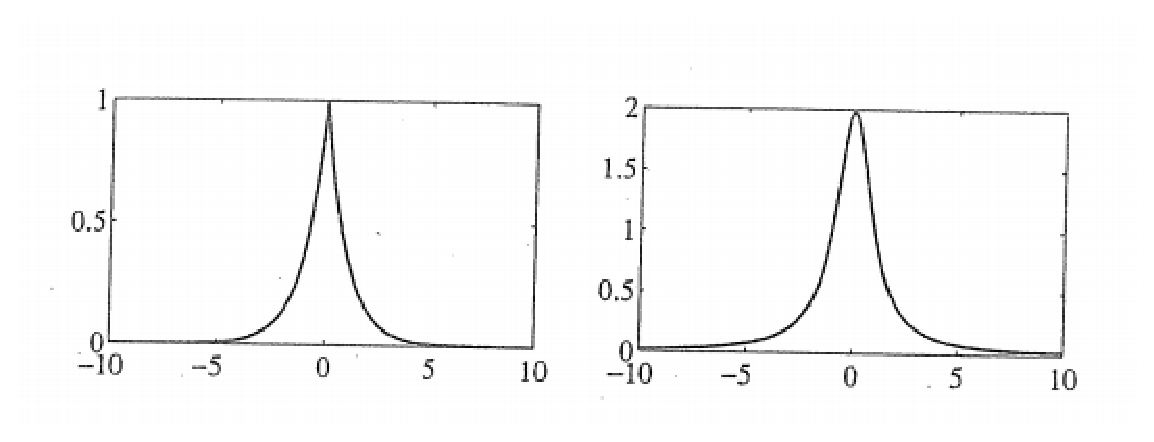
\includegraphics[width=0.7\linewidth]{TeX_files/Part02/chapter05/image/1}
	     	\caption{ $ \sigma=1 $ , $\alpha=1$的高斯马尔科夫过程中的自相关函数 $ R_{x}(\tau) $ 和频谱密度函数 $ S_{x}(\omega) $  }
	     \end{figure}
	      
	      
	      
	      我们假设 $ \varepsilon_{\tau} $ 是零均值的正态分布,并计算方差
	      
	     	\begin{equation}\label{5.20}
	     \begin{aligned}
	     E\left\lbrace\epsilon_{\tau}^{2} \right\rbrace &=E\left\lbrace(x(t+\tau)-e^{-\alpha|\tau|x(t)})^{2} \right\rbrace\\
	     &=E\left\lbrace x(t+\tau)^{2}-2e^{-\alpha|\tau|}x(t+\tau)x(t)+e^{-2\alpha|\tau|}x(t)^{2}\right\rbrace \\
	     &=\sigma^{2}-2\sigma^{2}e^{-\alpha|\tau|} +\sigma^{2}e^{-2\alpha|\tau|}\\
	     &=\sigma^{2}(1-e^{-2\alpha|\tau|}) 
	     \end{aligned}
	     \end{equation}
	      
	      我们假设 $ \epsilon_{\tau} $ 独立于 $ x(t) $ 。这个过程称为自回归。如果  $ \epsilon_{k}  $ 是i.i.d,我们在 $ k = 1, 2, 3,... $ 取样,这个过程被描述为 
	      
	     \begin{equation}\label{5.21}
	    x_{k}=px_{k-1} +\epsilon_{k}
	    \end{equation}
	     
	     其中采样间隔为 $ \tau=1 $ 时 $ p=e^{-\alpha} $。
	     
	     频谱密度 $ S_{x}(\omega) $  的逆变换重建了自相关
	     
	    	\begin{equation}\label{5.22}
	    R_{x}(\tau)=\frac{1}{2\pi}\int_{-\infty}^{+\infty}S_{x}(\omega)e^(j\omega\tau)d\omega
	    \end{equation}
	     
	     $ \tau=0 $ 时:
	     
	     \begin{equation}\label{5.23}
	     R_{x}(0)=E\left\lbrace x^{2}(t) \right] =\frac{{1}{2\pi}}\int_{-\infty}^{+\infty} s_{x}(\omega)d\omega
	     \end{equation}
	     当 $ R_{x}(\tau)=R_{x}(-\tau) $ 时我们同样得到 $ S_{x}(\omega)=S_{x}(-\omega) $ 。所以功率谱密度函数是关于 $ \omega $  的对称函数。
	    
	     \textbf{实例5.5}(高斯-马尔克夫过程)我们考虑频谱函数(5.19)
	     
	     \[ S_{x}(\omega)=\frac{2\sigma^{2}\alpha}{\alpha^{2}+\omega^{2}} \]	
	     
	     用(5.23)我们应该恢复  $ \sigma^{2} $,所以我们执行积分
	     	
	   	\begin{equation*}
	   \begin{aligned}
	   E\left\lbrace x^{2}\right\rbrace&=\frac{1}{2\pi}\int_{-\infty}^{+\infty}\frac{2\sigma^{2}\alpha}{\alpha^{2}+\omega^{2}}d\omega \\
	   &= \frac{\sigma^{2}\alpha}{\pi}\left\lbrace \frac{1}{\alpha}\arctan(\frac{\omega}{\alpha}) \right\rbrace_{-\infty}^{+\infty} =\sigma^{2}
	   \end{aligned}
	   \end{equation*}
	     
	     采用傅里叶变换的傅里叶逆变换,我们恢复了原始函数
	     
	   	\begin{figure}[h]
	   	\centering
	   	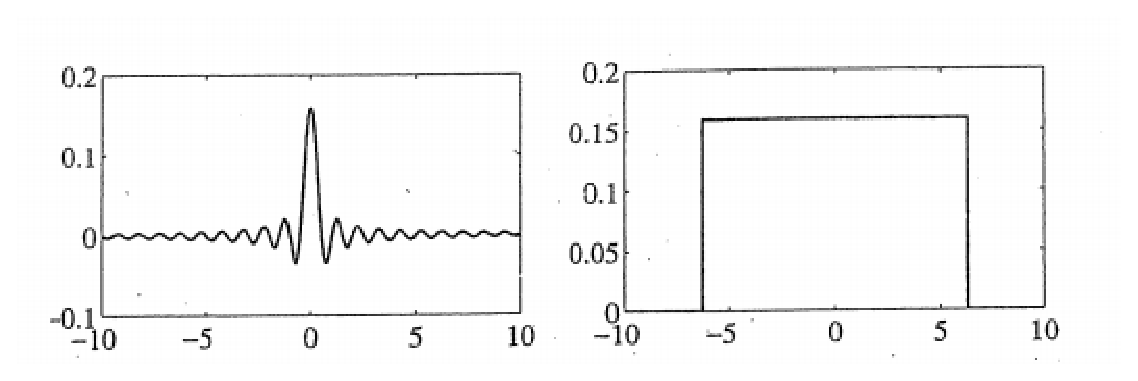
\includegraphics[width=0.7\linewidth]{TeX_files/Part02/chapter05/image/2}
	   	\caption{ 带限白噪声的自相关 $ R_{x}(\tau) $ 和频谱函数 $ S_{x}\omega) $}
	   \end{figure}
	     
	 
	     
	     我们想评价功率谱密度的解释。白噪声类似于无线电中的蜂鸣,它包含所有的音调(频率)。其功率谱密度函数是 $ S_{x}\omega) =$ 常数。 相反,纯余弦波形的功率谱密度具有作为功率谱密度的delta函数(实际上是两个delta函数,在 $ +\omega $ 和 $ -\omega $)。频谱密度反映了在信号 $ x(t) $ 的频率的组成。
	     下面的例子详细讨论了这个问题。
	     
	     \textbf{实例5.6}哪个自相关函数从 $ -\infty $ 到 $ +\infty $  对应于一个恒定的功率谱密度 $ S_{0} $?功率在所有频率上均匀分布。类似于白光的情况,这种随机过程称为白噪声:
	     
	     	$ R_{x}(\tau) =\frac{1}{2\pi}\int_{-\infty}^{+\infty}S_{0}e^{-j\omega\tau}d\omega=S_{0}\delta(\tau) $ 
	     	
	     	当$ \tau=0 $ , 由 $ \delta(\tau) $ 得出 $ R_{x}=S_{0}\delta(0)=\infty $. 这是 $ E\left\lbrace (x(t))^{2}\right\rbrace  $. 白噪声是一个理想化过程。
	     	
	     	声音的另一个特性是带宽,通常与系统的带宽相比噪声的带宽变宽。
	     	我们定义一个带宽受限的白噪声在有限频率范围内为常数,其他情况为0。
	     	
	     		\[ S(\omega) =\{ _{0,for|\omega|>2\pi W}^{A,for|\omega|<2\pi W} \]
	     	
	     	
	     	$ w $ 是以赫兹为单位的物理带宽。$ S(w) $ 的自相关是这个函数的逆变换,它产生了正弦函数 $ \frac{\sin x}{x} $。
	     	
	     		\[ R(\tau)=2WA\frac{\sin (2\pi W \tau)}{2\pi W \tau}\]
	     		
	     	这不是带宽受限,在有限的区间里同时成立 $ S(\omega) $  和 $ R(\omega) $  是不可能的。海森堡的不确定性原则给出了它们方差的精确限制 $ \sigma_{S}\sigma_{R} >\frac{1}{2} $。	
	     	
	     	图5.2描述了受限白噪声的自相关和频谱密度函数。当$\tau=\frac{1}{2W},\frac{2}{2W},\frac{3}{2W}... $时,函数  $ R_{x}(\tau) $ 为0.因此,如果该过程以2w样本/秒的Nyquistrate进行采样,则所得到的离散随机过程是不相关的。由于这简化了分析,所以经常做白色受限假设。
	     	
	     	\[ \textbf{Table 5.1} \quad System models of continuous random process \] 
	     	\[ \begin{tabular}{lcr}
	     	\hline
	     	Process\quad type & $ Autocorrelation\quad R_{x}(\tau) $ & $ Power \quad spectral \quad density S_{x}(\omega) $ \\
	     	\cline{1-3}
	     	White \quad noise &$  \sigma^{2}\delta(\tau) $  & $ \sigma^{2} $(constant)\\
	     	\cline{1-3}
	     	Random \quad walk&undefined&$ \sigma^{2}/\omega^{2} $\\
	     	\cline{1-3}
	     	Random \quad constant&$ \sigma^{2} $&$ 2\pi\sigma^{2}\delta(\omega) $\\
	     	\cline{1-3}
	     	Exponenitially\quad correlated &$ \sigma^{2}e^{-\alpha|\tau|} $,where\quad$  1/\alpha= $&$ \frac{2\sigma^{2}\alpha}{\omega^{2}+\alpha^{2}} $\\
	     	\cline{1-3}
	     	$ or\quad Gauss-Markov  $& $ correlation\quad time $& $ \quad $ \\
	     	\hline
	     	\end{tabular} \]      	
	     	
	     